\documentclass{article}
\usepackage[utf8]{inputenc}
\usepackage{geometry}
\usepackage{graphicx}
\usepackage{amsmath}
\usepackage{amsfonts}
\usepackage{amsthm}
\usepackage{amssymb}
\usepackage[most]{tcolorbox}
\usepackage{array}
\usepackage{latexsym}
\usepackage{alltt}
\usepackage{hyperref}
\usepackage{color, colortbl}
\usepackage{float}
\usepackage{pdfpages}
\usepackage{algpseudocode}
\usepackage{multicol}
\usepackage{multirow}
\usepackage{caption}
\usepackage{xparse}
\usepackage{setspace}
\usepackage{enumitem}
\usepackage{pdflscape}
% \usepackage{parskip}
\usepackage{blindtext}
\usepackage{forest}
% \usepackage[newfloat]{minted}
\usepackage{booktabs}


\geometry
{
  a4paper,
  left=12mm,
  right=12mm,
  top=12mm,
  bottom=15mm,
}

% mybox
\newtcolorbox{mybox}[3][]
{
  colframe = #2!25,
  colback  = #2!10,
  coltitle = #2!20!black,  
  title    = {#3},
  #1,
}

\definecolor{ex}{rgb}{1.00,0.65,0.00}
\definecolor{bg}{rgb}{0.95,0.95,0.95}
% \setminted
% {
% 	mathescape=true,
% 	xleftmargin=\parindent,
% 	bgcolor=bg,
% 	escapeinside=@@
% }

% \SetupFloatingEnvironment{listing}{name=Code}

% New environments that use mybox
\newcounter{example}[section]
\newenvironment{example}[1]{\begin{mybox}[breakable]{ex}{\refstepcounter{example}\textbf{Example \thesection.\theexample #1}}}{\end{mybox}}

\newcounter{definition}[section]
\newenvironment{definition}[1]{\refstepcounter{definition}\begin{mybox}[breakable]{blue}{\textbf{Definition \thesection.\thedefinition #1}}}{\end{mybox}}

\newcounter{theorem}[section]
\newenvironment{theorem}[1]{\begin{mybox}{red}{\refstepcounter{theorem}\textbf{Theorem \thesection.\thetheorem #1}}}{\end{mybox}}

\newenvironment{formula}[1]{\begin{mybox}{cyan}{\textbf{#1}}}{\end{mybox}}

% Changing maketitle
\makeatletter         
\renewcommand\maketitle{
{\raggedright % Note the extra {
\begin{center}
{\Large \bfseries \@title}\\[2ex] 
{\large \@author \ - \@date}\\[2ex]
\end{center}}} % Note the extra }
\makeatother

% \onehalfspacing % adjust spacing
\setlength{\parskip}{0.5\baselineskip}

% macros
\newcommand{\prob}[1]{\textbf{\textit{P}}\left\{#1\right\}}
\newcommand{\expc}[1]{\mathbf{E}\left(#1\right)}
\newcommand{\expcs}[1]{\mathbf{E}^2\left(#1\right)}
\newcommand{\var}[1]{\text{Var}\left( #1 \right)}
\newcommand{\ra}{\rightarrow}
\newcommand{\Ra}{\Rightarrow}
\newcommand{\R}[2]{\tikz [remember picture,overlay] \node (#1) {#2};}

\def\circtxt#1{$\mathalpha \bigcirc \mkern-13mu \mathtt #1$}
\def\smiley{\textcircled{\scriptsize $\mkern3mu\ddot{\ } \mkern-15mu \smallsmile$}}

\NewDocumentCommand{\dsum}{%
    e{^_}
}{%
  {% 
    \displaystyle\sum
    \IfValueT{#1}{^{#1}}
    \IfValueT{#2}{_{#2}}
  }
}%

% maketitle variables
\title{CENG 232 - Chapter 7: Memory and Programmable Logic}
\author{Burak Metehan Tunçel}
\date{June 2022}

\begin{document}

\maketitle

\begin{multicols*}{2}
\setlength{\columnsep}{1.5cm}
\setlength{\columnseprule}{0.2pt}

\section{Introduction}
\label{sec:introduction}

A memory unit is a device to which binary information is transferred for storage and from which information is retrieved when needed for processing. When data processing takes place, information from memory is transferred to selected registers in the processing unit. A \textit{memory unit} is a \textit{collection of cells capable of storing a large quantity of binary information}.

There are two types of memories that are used in digital systems: 
\begin{itemize}
  \item random-access memory (RAM)
  \item read-only memory (ROM)
\end{itemize}
\noindent RAM stores new information for later use. The process of storing new information into memory is referred to as a memory \textit{write} operation. The process of transferring the stored information out of memory is referred to as a memory \textit{read} operation.

RAM can perform \textit{both write and read} operations. ROM can \textit{perform only the read} operation. This means that suitable binary information is already stored inside memory and can be retrieved or read at any time. However, that information cannot be altered by writing.

ROM is a \textit{programmable logic device} (\textbf{PLD}). The binary information that is stored within such a device is specified in some fashion and then embedded within the hardware in a process referred to as programming the device. The word ``programming'' here refers to a hardware procedure, which specifies the bits that are inserted into the hardware configuration of the device.

Figure 1 shows the conventional and array logic symbols for a multiple input OR gate.
\begin{figure}[H]
  \centering
  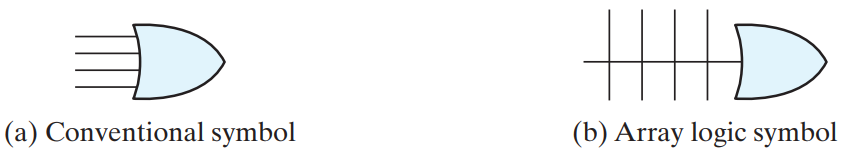
\includegraphics[width=\linewidth]{img/fig-7.1.png}
  \caption{Conventional and array logic diagrams for OR gate}
  \label{fig:7.1}
\end{figure}


\section{Random-Access Memory}
\label{sec:ram}

\textit{A memory unit is a collection of storage cells}, together with associated circuits needed to transfer information into and out of a device. The architecture of memory is such that information can be selectively retrieved from any of its internal locations. The time it takes to transfer information to or from any desired random location is always the same -hence the name random-access memory, abbreviated RAM. In contrast, the time required to retrieve information that is stored on magnetic tape depends on the location of the data.

A memory unit stores binary information in groups of bits called \textbf{\textit{words}}. A \textit{word in memory is a set of bits that move in and out of storage as a unit}. A memory word is a group of 1's and 0's and may represent a number, an instruction, one or more alphanumeric characters, or any other binary-coded information. \textit{A group of 8 bits is called a byte}. Most computer memories use words that are multiples of 8 bits in length. The capacity of a memory unit is usually stated as the total number of bytes that the unit can store.

Communication between memory and its environment is achieved through \textit{data input} and \textit{output lines}, \textit{address selection lines}, and \textit{control lines} that specify the direction of transfer. A block diagram of a memory unit is shown in Fig. 2. 
\begin{figure}[H]
  \centering
  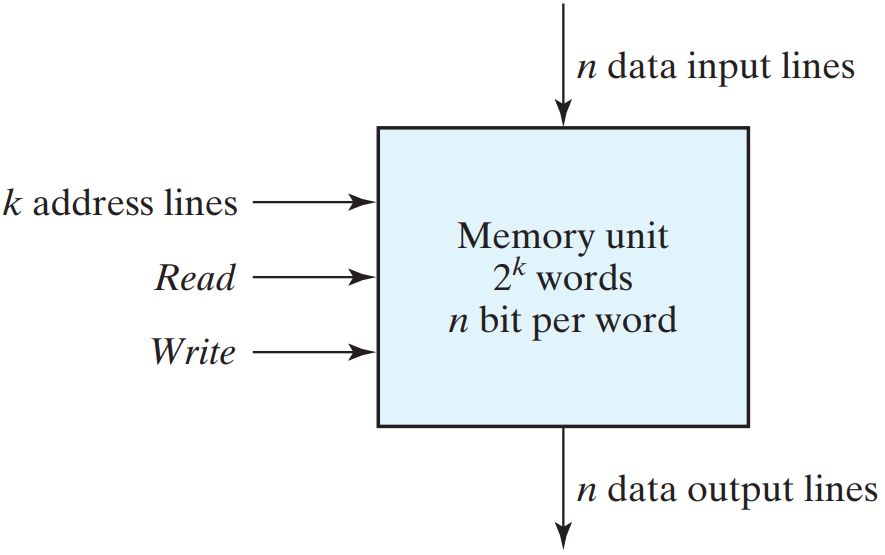
\includegraphics[width=\linewidth]{img/fig-7.2.png}
  \caption{Block diagram of a memory unit}
  \label{fig:7.2}
\end{figure}
\noindent The $n$ data input lines provide the information to be stored in memory, and the $n$ data output lines supply the information coming out of memory. The $k$ address lines specify the particular word chosen among the many available. The two control inputs specify the direction of transfer 
desired: The \textit{Write} input causes binary data to be transferred into the memory, and the \textit{Read} input causes binary data to be transferred out of memory.

The \textit{memory unit is specified by the number of words it contains and the number of bits in each word} ($cell\_size \times word\_size$). The address lines select one particular word. Each word in memory is assigned an identification number, called an address, starting from 0 up to $2^{k - 1}$, where $k$ is the number of address lines.v

The $1K \times 16$ memory of Fig. 3 has 10 bits in the address and 16 bits in each word. Figure 3 shows possible contents of the first three and the last three words of this memory. Each word contains 16 bits that can be divided into two bytes.
\begin{figure}[H]
  \centering
  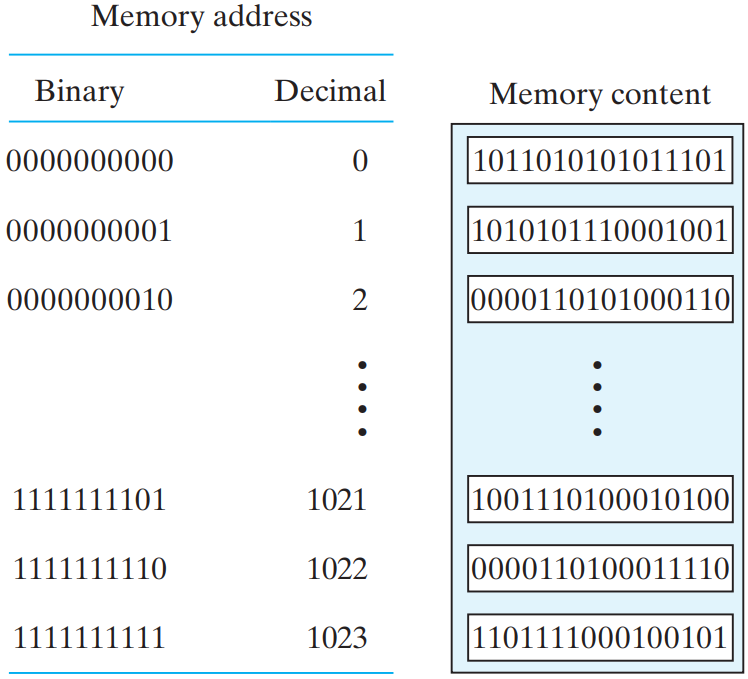
\includegraphics[width=\linewidth]{img/fig-7.3.png}
  \caption{Contents of a $1024 \times 16$ memory}
  \label{fig:7.3}
\end{figure}
\textit{The number of address bits needed in a memory is dependent on the total number of words that can be stored in the memory and is independent of the number of bits in each word}. The number of bits in the address is determined from the relationship $2^k \geq m$, where $m$ is the total number of words and $k$ is the number of address bits needed to satisfy the relationship.


\subsection{Write and Read Operations}
\label{subsec:write-read-operations}

The two operations that RAM can perform are the write and read operations. The write signal specifies a transfer-in operation and the read signal specifies a transfer-out operation. On accepting one of these control signals, the internal circuits inside the memory provide the desired operation.

The steps that must be taken for the purpose of transferring a new word to be stored into memory are as follows:
\begin{enumerate}
  \item Apply the binary address of the desired word to the address lines.
  \item Apply the data bits that must be stored in memory to the data input lines.
  \item Activate the \textit{write} input.
\end{enumerate}
\noindent The memory unit will then take the bits from the input data lines and store them in the word specified by the address lines.

The steps that must be taken for the purpose of transferring a stored word out of memory are as follows:
\begin{enumerate}
  \item Apply the binary address of the desired word to the address lines.
  \item Activate the read input.
\end{enumerate}
The memory unit will then take the bits from the word that has been selected by the address and apply them to the output data lines. The contents of the selected word do not change after the read operation, that is, the read operation is nondestructive.

Most integrated circuits provide two other control inputs: One input selects the unit and the other determines the operation. The memory operations that result from these control inputs are specified in Table 7.1.
\begin{figure}[H]
  \centering
  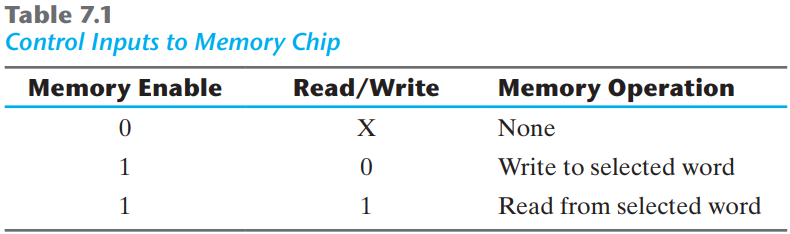
\includegraphics[width=\linewidth]{img/table-7.1.png}
  \label{table:7.1}
\end{figure}


\subsection{Timing Waveforms}
\label{subsec:timing-waveforms}

The operation of the memory unit is controlled by an external device such as a central processing unit (CPU). The CPU is usually synchronized by its own clock. The memory, however, does not employ an internal clock. Instead, its read and write operations are specified by control inputs.

The \textbf{\textit{access time}} of memory is the \textit{time required to select a word and read it}. The \textit{\textbf{cycle time}} of memory is the \textit{time required to complete a write operation}.

The CPU must provide the memory control signals in such a way as to synchronize its internal clocked operations with the read and write operations of memory. This means that the access time and cycle time of the memory must be within a time equal to a fixed number of CPU clock cycles.

The memory timing shown in Fig. 4 is for a CPU with a 50 MHz clock and a memory with 50 ns maximum cycle time. The write cycle in part (a) shows three 20 ns cycles: $T_1$, $T_2$, and $T_3$. For a write operation, the CPU must provide the address and input data to the memory. This is done at the beginning of $T_1$.

The memory enable and the read/write signals must be activated after the signals in the address lines are stable in order to avoid destroying data in other memory words. The memory enable signal switches to the high level and the read/write signal switches to the low level to indicate a write operation.

The two control signals must stay active for at least 50 ns. The address and data signals must remain stable for a short time after the control signals are deactivated. At the completion of the third clock cycle, the memory write operation is completed and the CPU can access the memory again with the next $T_1$ cycle.

The read cycle shown in Fig. 4(b) has an address for the memory provided by the CPU. The memory enable and read/write signals must be in their high level for a read operation. The memory places the data of the word selected by the address into the output data lines within a 50 ns interval (or less) from the time that the memory enable is activated. The CPU can transfer the data into one of its internal registers during the negative transition of $T_3$. The next $T_1$ cycle is available for another memory request.
\vspace*{\fill}
\columnbreak
\begin{figure}[H]
  \centering
  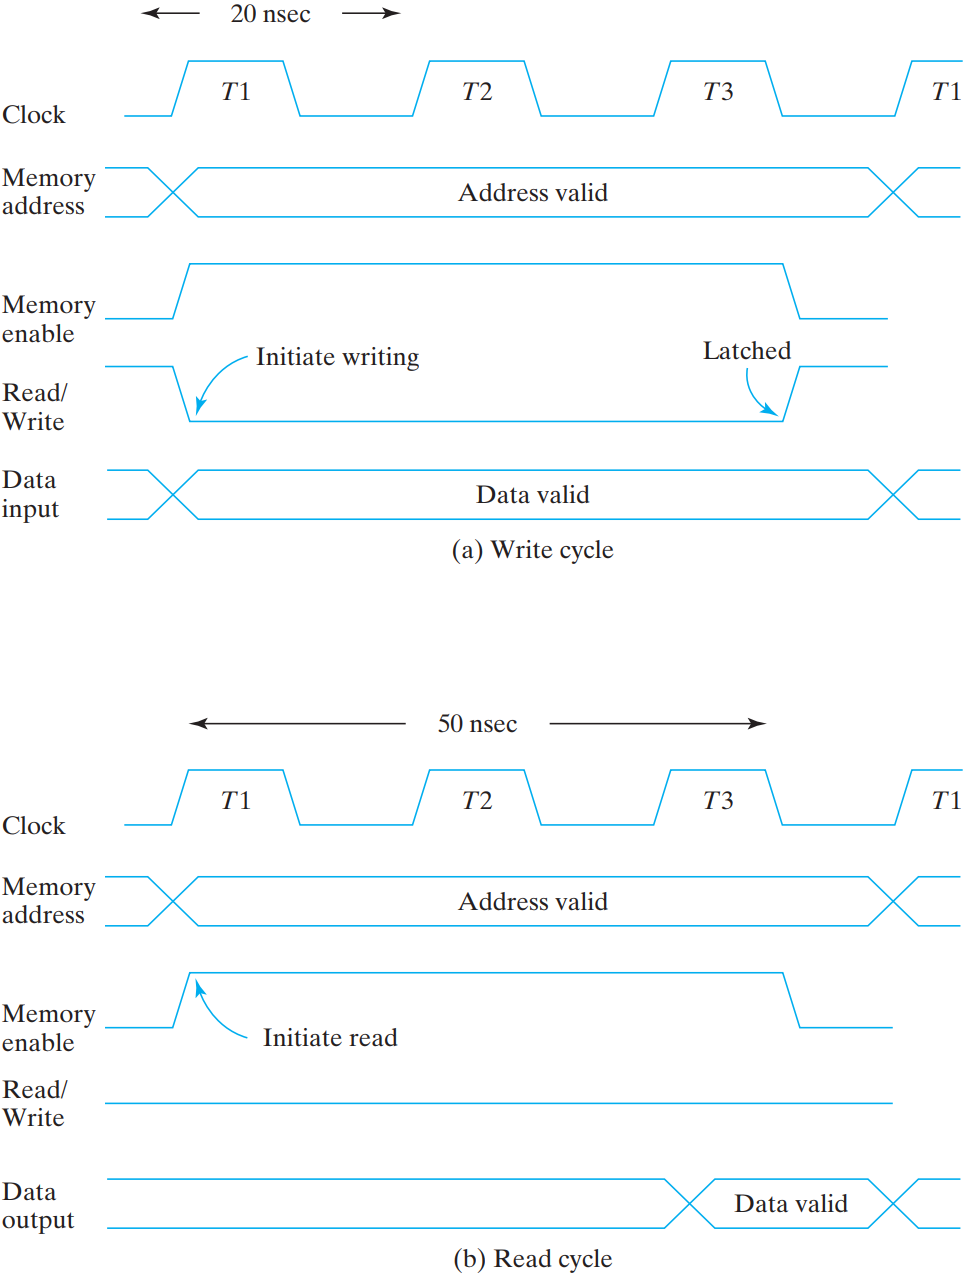
\includegraphics[width=\linewidth]{img/fig-7.4.png}
  \caption{Memory cycle timing waveforms}
  \label{fig:7.4}
\end{figure}


\subsection{Types of Memories}
\label{subsec:types-of-memories}

Integrated circuit RAM units are available in two operating modes: \textit{static} and \textit{dynamic}. 
\begin{itemize}
  \item \textit{\textbf{Static RAM}} (\textit{SRAM}) consists essentially of \textit{internal latches that store the binary information}. The stored information remains valid as long as power is applied to the unit.
  \item \textit{\textbf{Dynamic RAM}} (\textit{DRAM}) \textit{stores the binary information in the form of electric charges on capacitors} provided inside the chip by MOS transistors. The stored charge on the capacitors tends to discharge with time, and the capacitors must be periodically recharged by \textit{refreshing} the dynamic memory.
\end{itemize} 

Refreshing is done by cycling through the words every few milliseconds to restore the decaying charge. DRAM offers reduced power consumption and larger storage capacity in a single memory chip. SRAM is easier to use and has shorter read and write cycles.

The reason why latches are used in SRAM is that a latch can be made with only two NAND or two NOR gates, but a flip-flop requires at least twice that much hardware. Also, in general, smaller is faster, cheaper and requires less power.

Dynamic RAMs tend to be physically smaller than static RAMs. So, this means dynamic RAM is cheaper and denser—more bits can be stored in the same physical area. DRAM offers reduced power consumption and larger storage capacity in a single memory chip.


\section{Memory Decoding}
\label{sec:memory-decoding}

In addition to requiring storage components in a memory unit, there is a need for decoding circuits to select the memory word specified by the input address.

\subsection{Internal Construction}
\label{subsec:internal-construction}

The internal construction of a RAM of $m$ words and $n$ bits per word consists of $m \times n$ binary storage cells and associated decoding circuits for selecting individual words. The binary storage cell is the basic building block of a memory unit. The equivalent logic of a binary cell that stores one bit of information is shown in Fig. 5.
\begin{figure}[H]
  \centering
  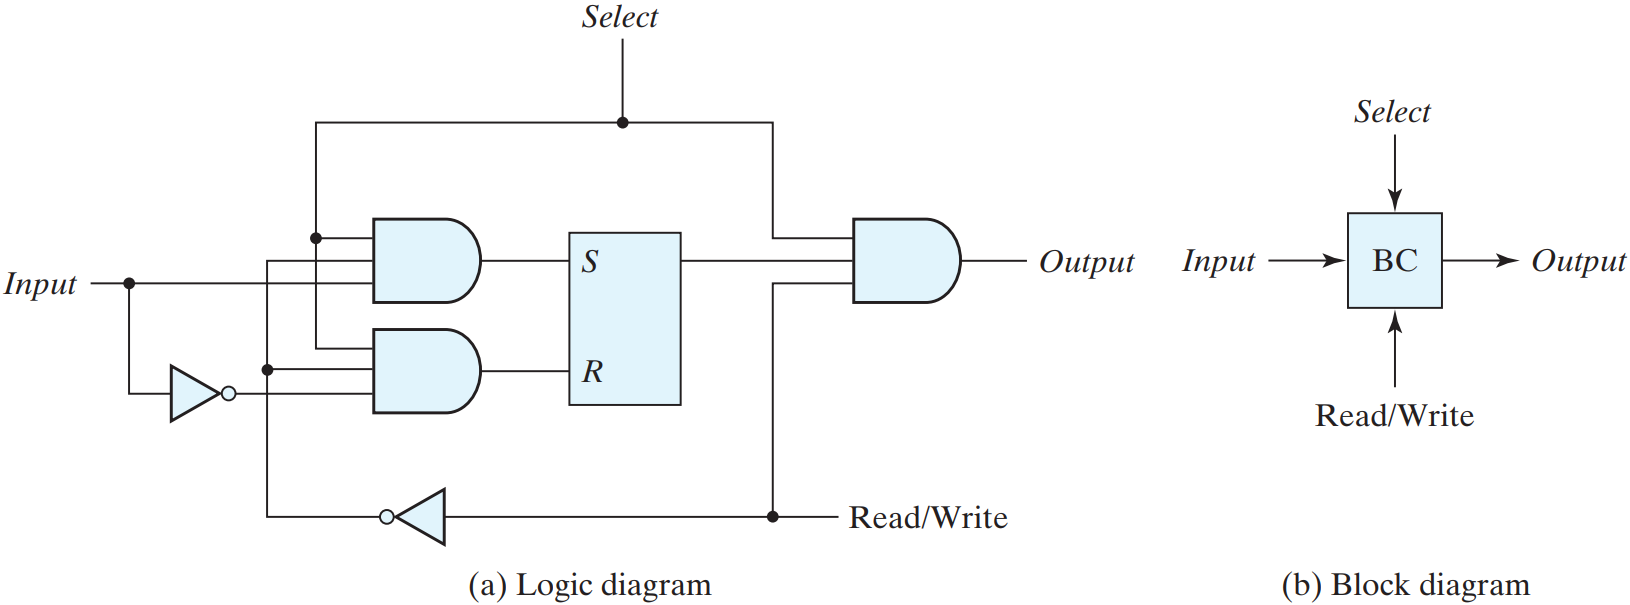
\includegraphics[width=\linewidth]{img/fig-7.5.png}
  \caption{Memory cell}
  \label{fig:7.5}
\end{figure}

Actually, the cell is an electronic circuit with \textit{four to six transistors}. Nevertheless, it is possible and convenient to model it in terms of logic symbols. A binary storage cell must be very small in order to be able to pack as many cells as possible in the small area available in the integrated circuit chip. 

The binary cell stores one bit in its internal latch. The select input enables the cell for reading or writing, and the read/write input determines the operation of the cell when it is selected.
\begin{itemize}
  \item \textit{Read}: A 1 in the read/write input provides the read operation by forming a path from the latch to the output terminal.
  \item \textit{Write}: A 0 in the read/write input provides the write operation by forming a path from the input terminal to the latch.
\end{itemize}

The logical construction of a small RAM is shown in Fig. 6. This RAM consists of four words of four bits each and has a total of 16 binary cells. The small blocks labeled BC represent the binary cell with its three inputs and one output, as specified in Fig. 5(b). 

A memory with four words needs two address lines. The two address inputs go through a $2 \times 4$ decoder to select one of the four words. The decoder is enabled with the memory enable input. When the memory enable is 0, all outputs of the decoder are 0 and none of the memory words are selected. With the memory select at 1, one of the four words is selected, dictated by the value in the two address lines. Once a word has been selected, the read/write input determines the operation.

\end{multicols*}

\begin{figure}[H]
  \centering
  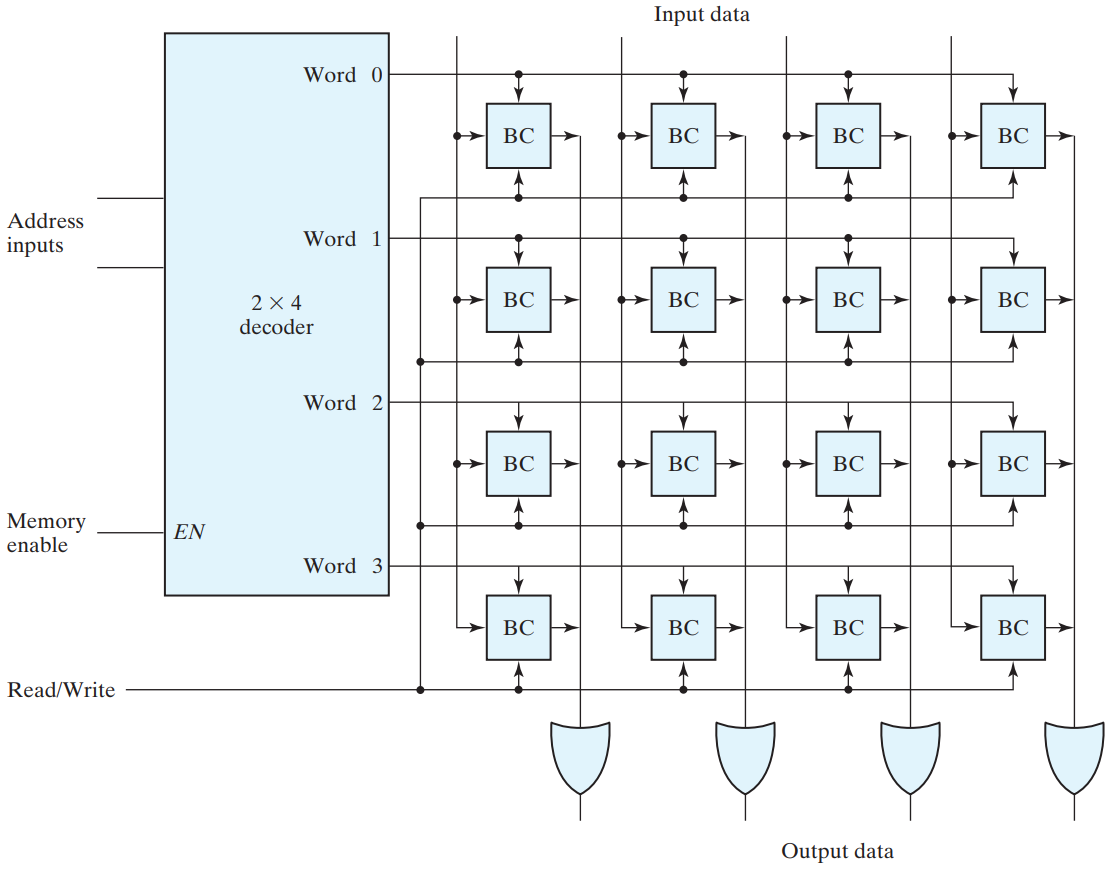
\includegraphics[width=\linewidth]{img/fig-7.6.png}
  \caption{Diagram of a $4 \times 4$ RAM}
  \label{fig:7.6}
\end{figure}

\begin{multicols}{2}
\setlength{\columnsep}{1.5cm}
\setlength{\columnseprule}{0.2pt}

\begin{itemize}
  \item During the read operation, the four bits of the selected word go through OR gates to the output terminals.
  \item During the write operation, the data available in the input lines are transferred into the four binary cells of the selected word.
\end{itemize}

The binary cells that are not selected are disabled, and their previous binary values remain unchanged. When the memory select input that goes into the decoder is equal to 0, none of the words are selected and the contents of all cells remain unchanged regardless of the value of the read/write input.

A memory with $2^k$ words of $n$ bits per word requires $k$ address lines that go into a $k \times 2^k$ decoder. Each one of the decoder outputs selects one word of $n$ bits for reading or writing.

\vspace*{\fill}
\columnbreak

\subsection{Coincident Decoding}
\label{subsec:coincident-decoding}

A decoder with $k$ inputs and $2^k$ outputs requires $2^k$ AND gates with $k$ inputs per gate. The total number of gates and the number of inputs per gate can be reduced by employing two decoders in a two-dimensional selection scheme. The basic idea in two-dimensional decoding is to arrange the memory cells in an array that is close as possible to square. In this configuration, two $k/2$-input decoders are used instead of one $k$-input decoder. One decoder performs the row selection and the other the column selection in a two-dimensional matrix configuration.

The two-dimensional selection pattern is demonstrated in Fig. 7 for a 1K-word memory. Instead of using a single $10 \times 1,024$ decoder, we use two $5 \times 32$ decoders. With the single decoder, we would need 1,024 AND gates with 10 inputs in each. In the two-decoder case, we need 64 AND gates with 5 inputs in each. The five most significant bits of the address go to input $X$ and the five least significant bits go to input $Y$.

Each word within the memory array is selected by the coincidence of one $X$ line and one $Y$ line. Thus, each word in memory is selected by the coincidence between 1 of 32 rows and 1 of 32 columns, for a total of 1,024 words. Note that each intersection represents a word that may have any number of bits.
\end{multicols}

\begin{figure}[H]
  \centering
  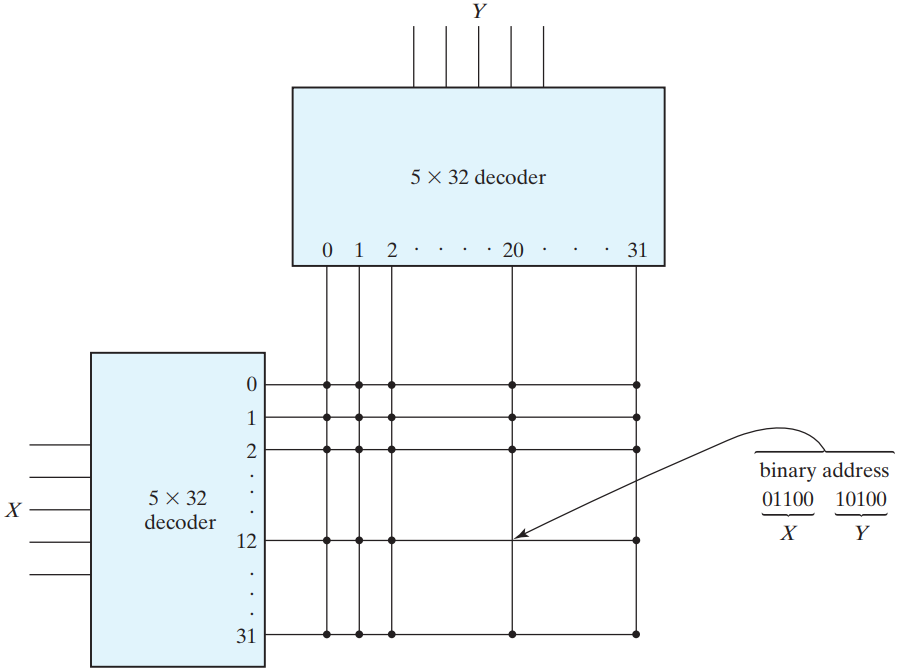
\includegraphics[width=\linewidth]{img/fig-7.7.png}
  \caption{Two-dimensional decoding structure for a 1K-word memory}
  \label{fig:7.7}
\end{figure}

\begin{multicols}{2}
\setlength{\columnsep}{1.5cm}
\setlength{\columnseprule}{0.2pt}

\subsection{Address Multiplexing}
\label{subsec:address-multiplexing}

The SRAM memory cell modeled in Fig. 5 typically contains six transistors. In order to build memories with higher density, it is necessary to reduce the number of transistors in a cell. The DRAM cell contains a single MOS transistor and a capacitor. The charge stored on the capacitor discharges with time, and the memory cells must be periodically recharged by refreshing the memory. 

Because of their simple cell structure, \textit{DRAMs typically have four times the density of SRAMs}. This allows four times as much memory capacity to be placed on a given size of chip. The cost per bit of DRAM storage is three to four times less than that of SRAM storage. A further (operational) cost savings is realized because of the lower power requirement of DRAM cells. 

These advantages make DRAM the preferred technology for large memories in personal digital computers. DRAM chips are available in capacities from 64K to 512M bits. Most DRAMs have a 1-bit word size, so several chips have to be combined to produce a larger word size.

\vspace*{\fill}
\columnbreak

Because of their large capacity, the address decoding of DRAMs is arranged in a two-dimensional array, and larger memories often have multiple arrays. To reduce the number of pins in the IC package, designers utilize address multiplexing whereby one set of address input pins accommodates the address components. In a two-dimensional array, the address is applied in two parts at different times, with the row address first and the column address second. Since the same set of pins is used for both parts of the address, the size of the package is decreased significantly.

We will use a 64K-word memory to illustrate the address-multiplexing idea. A diagram of the decoding configuration is shown in Fig. 8. The memory consists of a two-dimensional array of cells arranged into 256 rows by 256 columns, for a total of $2^8 \times 2^8 = 2^{16} = 64K$ words. There is a single data input line, a single data output line, and a read/write control, as well as an eight-bit address input and two address strobes, the latter included for enabling the row and column address into their respective registers. The row address strobe (RAS) enables the eight-bit row register, and the column address strobe (CAS) enables the eight-bit column register. The bar on top of the name of the strobe symbol indicates that the registers are enabled on the zero level of the signal.

\end{multicols}

\begin{figure}[H]
  \centering
  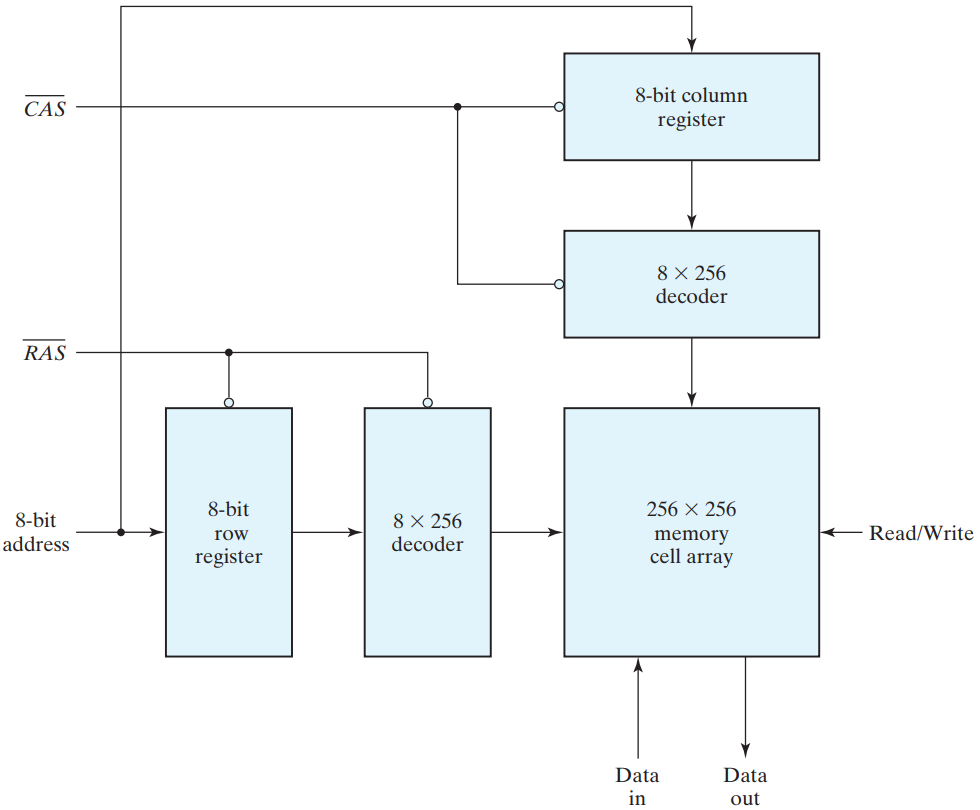
\includegraphics[width=\linewidth]{img/fig-7.8.png}
  \caption{Address multiplexing for a 64K DRAM}
  \label{fig:7.8}
\end{figure}

\begin{multicols}{2}
\setlength{\columnsep}{1.5cm}
\setlength{\columnseprule}{0.2pt}

\end{multicols}

\end{document}
